
\subsubsection{5.1 Cohort Construction}

Of the WildChat-1M corpus, 27,902 IP-hash pseudonymized users satisfy the $\geq 3$ monthly bin criterion with $\geq 50$ users per bin in the h-e1-v2 analysis. The effective analysis window is 13 monthly bins from April 2023 through April 2024. Figure 3 shows the retention funnel.

\begin{figure}[htbp]
\centering
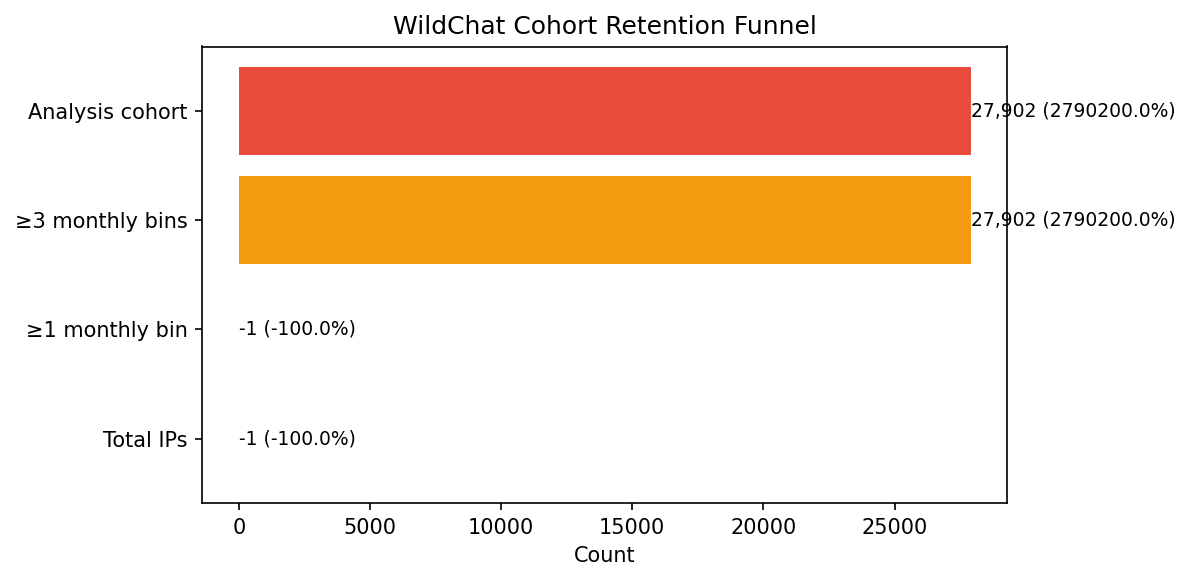
\includegraphics[width=\columnwidth]{figures/fig3_cohort_funnel.png}
\caption{Cohort Retention Funnel}
\label{fig:fig3_cohort_funnel}
\end{figure}

\textbf{Figure 3.} WildChat-1M retention funnel: all users $\rightarrow$ users with $\geq 1$ monthly bin $\rightarrow$ users with $\geq 3$ monthly bins $\rightarrow$ analysis cohort (n = 27,902).

Monthly cohort sizes range from approximately 1,246 users \citep{April2023} to approximately 2,986 users \citep{November2023}, as shown in Table 2 below.

\subsubsection{5.2 Gate Evaluation}

The pre-specified gate criterion requires $\geq 2$ of 3 proxies to achieve |$\tau | \geq$ 0.2 with p < 0.05. Table 1 reports full results.

\textbf{Table 1.} Mann-Kendall gate evaluation for all three behavioral proxies (h-e1-v2). p-values reported to 4 decimal places where available; significance notation p < 0.001 used in abstract and conclusion for conciseness.

\begin{table*}[htbp]
\centering
\resizebox{\dimexpr 2\columnwidth+\columnsep\relax}{!}{%
\begin{tabular}{lllllll}
\toprule
Proxy & $\tau$ & 95\% Bootstrap CI & p & ACF lag-1 & Method & Gate Result \\
\midrule
P1: Prompt token count & **+0.744** & [0.415, 0.972] & **0.0005** & 0.634 & Hamed-Rao & FAIL (direction)† \\
P2: Vote entropy & N/A & N/A & N/A & N/A & --- & FAIL (no data) \\
P3: Correction freq. & 0.051 & [$-0.441$, 0.536] & 0.855 & 0.168 & Hamed-Rao & FAIL \\
\bottomrule
\end{tabular}
}
\end{table*}

†P1 achieves statistical significance (p = 0.0005, |$\tau |$ = 0.744 >> 0.2 threshold) but fails the gate because $\tau$ > 0 contradicts the BAA directional prediction of $\tau$ < 0. This is a direction failure, not a significance failure.

\textbf{Gate result: n\_significant = 1/3. Gate FAILED (threshold: $\geq 2/3)$.}

The gate failure does not eliminate the substantive empirical finding: the positive trend in prompt length is the key result of the study, and it directly contradicts the BAA directional prediction.

\begin{figure}[htbp]
\centering
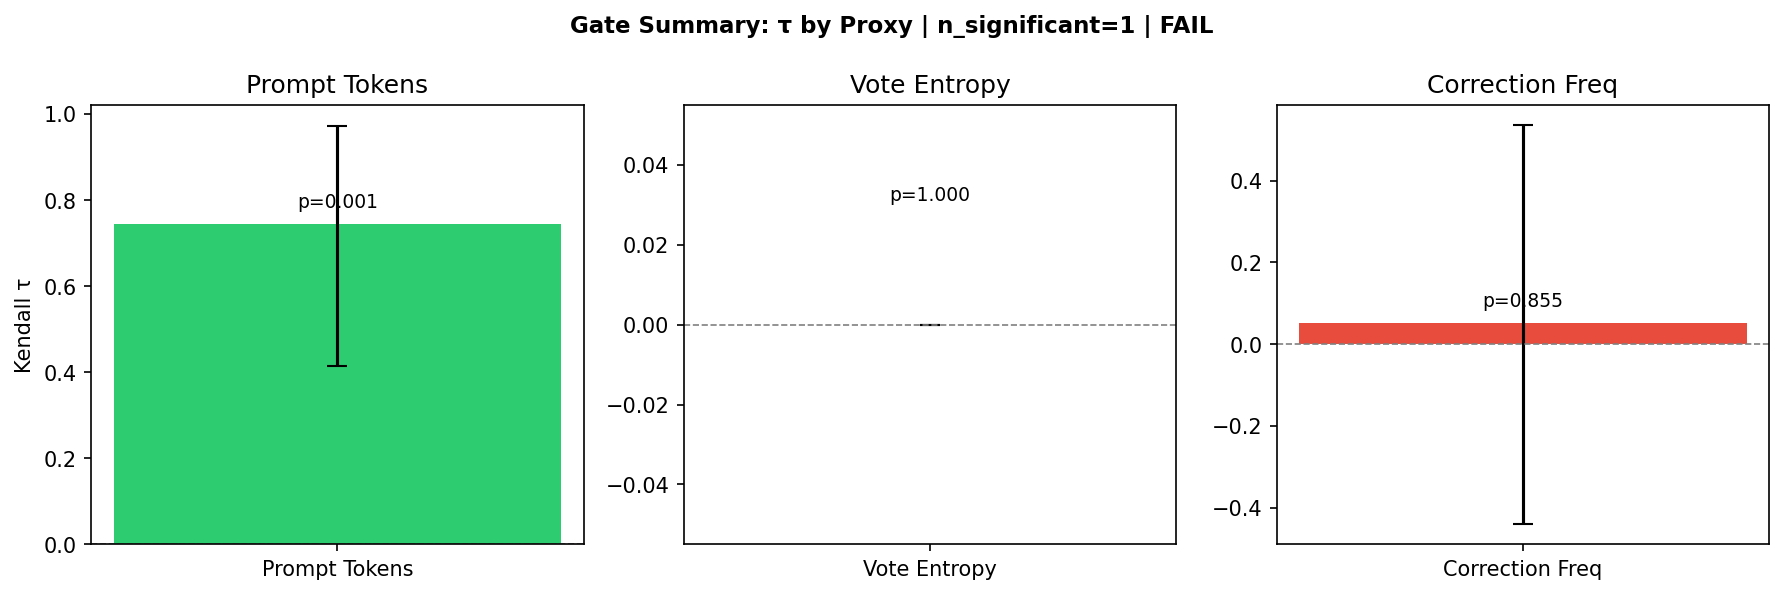
\includegraphics[width=\columnwidth]{figures/fig1_gate_summary.png}
\caption{Gate Summary}
\label{fig:fig1_gate_summary}
\end{figure}

\textbf{Figure 1.} Kendall $\tau \pm$ 95\% bootstrap CI for all three behavioral proxies. PASS/FAIL color coding reflects gate criterion (|$\tau | \geq$ 0.2, p < 0.05). P1 achieves significance but fails on direction; P2 is not computed; P3 shows no detectable signal.

\subsubsection{5.3 Proxy 1: Strong Positive Trend}

\textbf{Returning WildChat users' prompt length increases significantly over 2023--2024 ($\tau$ = +0.744, 95\% CI [0.415, 0.972], p = 0.0005).} The cohort-level mean prompt token count grows from approximately 180 tokens \citep{April2023} to approximately 832 tokens \citep{April2024}, a 4.$6\times$ increase in cohort mean over 13 months (this is aggregate cohort-mean growth; individual-level trajectories are not measured). The ACF lag-1 = 0.634 confirms that the Hamed-Rao correction is necessary; the result remains significant after this correction.

The 95\% bootstrap CI [0.415, 0.972] does not overlap $\tau$ = 0. The positive direction is consistent across both experiment rounds: h-e1 yields $\tau$ = +0.564 (p = 0.007, n = 6,769 returning users); h-e1-v2 yields $\tau$ = +0.744 (p = 0.0005, n = 27,902 returning users).

\textbf{This result is opposite to the BAA directional prediction ($\tau$ < 0).} The BAA framework predicts declining prompt complexity as AI quality improves; the observed trend is strongly positive.

\begin{figure}[htbp]
\centering
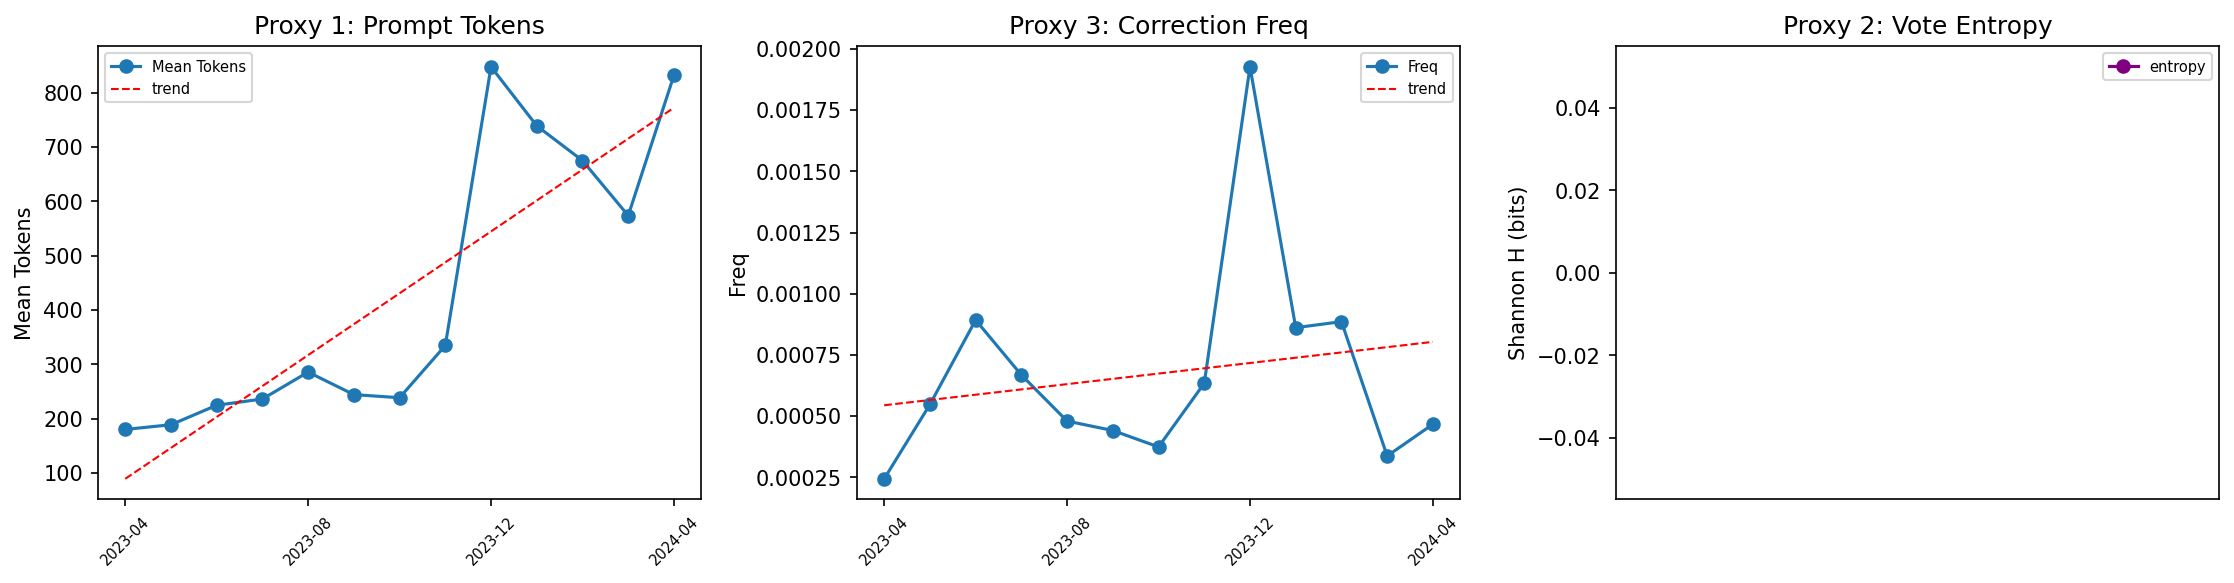
\includegraphics[width=\columnwidth]{figures/fig2_proxy_timeseries.png}
\caption{Proxy Time Series}
\label{fig:fig2_proxy_timeseries}
\end{figure}

\textbf{Figure 2.} Monthly time series of Proxy 1 (prompt token count, left axis) and Proxy 3 (correction frequency, right axis) for the returning-user cohort (April 2023--April 2024). Proxy 1 shows a strong positive monotonic trend; Proxy 3 fluctuates near zero with no detectable trend.

\subsubsection{5.4 Proxy 2: Not Computed}

LMSYS primary dataset access-gated. The fallback dataset (\texttt{lmsys/lmsys-arena-human-preference-55k}) contains no timestamp field, making temporal binning impossible. Vote entropy could not be computed from any publicly available data source. The entropy computation logic was implemented and verified on synthetic data in the smoke test suite; the failure is infrastructural, not methodological.

\subsubsection{5.5 Proxy 3: No Detectable Signal}

Correction/negation frequency: $\tau$ = 0.051, 95\% CI [$-0.441$, 0.536], p = 0.855. The empirical monthly base rate is approximately 0.05\% of turns. The Mann-Kendall test has negligible statistical power over a near-zero series. The proxy fails because explicit verbal corrections are extremely rare in naturalistic AI interaction; the regex pattern is too restrictive to capture the full range of correction behavior.

\subsubsection{5.6 Monthly Cohort Statistics (h-e1-v2)}

Table 2 reports the monthly cohort sizes and prompt token means from the authoritative h-e1-v2 analysis. Full data are available in \texttt{results/wildchat\textbackslash \_monthly.csv}.

\textbf{Table 2.} Monthly cohort statistics (h-e1-v2). Values from \texttt{h-e1-v2/results/wildchat\textbackslash \_monthly.csv}.

\begin{table}[htbp]
\centering
\resizebox{\columnwidth}{!}{%
\begin{tabular}{lll}
\toprule
Monthly Bin & Cohort Size & Mean Prompt Tokens \\
\midrule
2023-04 & 1,246 & 180.1 \\
2023-05 & 2,157 & 188.7 \\
2023-06 & 2,404 & 224.6 \\
2023-07 & 2,541 & 236.1 \\
2023-08 & 2,566 & 285.7 \\
2023-09 & 2,701 & 244.2 \\
2023-10 & 2,550 & 238.5 \\
2023-11 & 2,986 & 334.7 \\
2023-12 & 2,065 & 848.1 \\
2024-01 & 1,380 & 739.3 \\
2024-02 & 1,630 & 675.3 \\
2024-03 & 1,941 & 574.0 \\
2024-04 & 1,735 & 832.4 \\
\bottomrule
\end{tabular}
}
\end{table}

The sharp increase in mean prompt tokens between 2023-11 and 2023-12 (from 334.7 to 848.1) coincides with a reduction in cohort size (2,986 to 2,065 users), suggesting compositional changes in the retained cohort during this period. The cause of this shift is not determined.

\subsubsection{5.7 Internal Replication}

h-e1-v2 ($\tau$ = +0.744, n = 27,902) replicates the direction and significance of h-e1 ($\tau$ = +0.564, n = 6,769). The cohort size difference (~4.$1\times )$ reflects the tokenization method difference: h-e1 used a word-count approximation (words $\times$ 1.3); h-e1-v2 used tiktoken cl100k\_base. Because the tokenization method differs, the two rounds should be understood as methodological variants rather than identical replications; their agreement on direction ($\tau$ > 0, p < 0.05) is nonetheless informative.

